\documentclass[10pt]{article}

\usepackage[top=0.5in, bottom=0.5in, left=0.6in, right=0.6in]{geometry}
\usepackage{tikz}
\usetikzlibrary{positioning}
\usepackage{enumitem}
\usepackage{graphicx}
\usepackage{tgheros}
\usepackage{xcolor}
\renewcommand*{\familydefault}{\sfdefault}

\setlength{\parskip}{0pt}

% Change this value to resize the grade circle on the quiz header.
\newlength{\gradeCircleRadius}
\setlength{\gradeCircleRadius}{0.35in}

% Set this to the letter identifying this quiz version (e.g. A, B).
\newcommand{\quizVersion}{A}

% Solution text (answers, derivation steps) is shown in red throughout this guide.
\newcommand{\sol}[1]{\textcolor{red}{#1}}

% Reference diagrams of the USB and CAN frame structures, shown below each
% waveform (not to scale) to help students locate fields in the questions.
\newcommand{\usbFrameDiagram}{%
\begin{center}
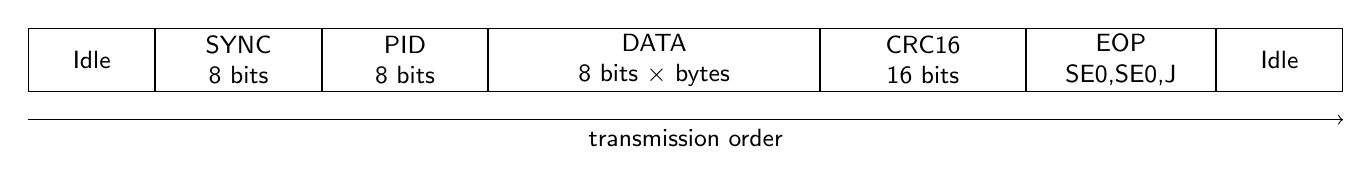
\begin{tikzpicture}[field/.style={draw, minimum height=0.8cm, align=center, font=\small, inner sep=2pt}]
\node[field, minimum width=1.6cm] (idle1) {Idle};
\node[field, minimum width=2.1cm, right=0pt of idle1] (sync) {SYNC\\8 bits};
\node[field, minimum width=2.1cm, right=0pt of sync] (pid) {PID\\8 bits};
\node[field, minimum width=4.2cm, right=0pt of pid] (data) {DATA\\8 bits $\times$ bytes};
\node[field, minimum width=2.6cm, right=0pt of data] (crc) {CRC16\\16 bits};
\node[field, minimum width=2.4cm, right=0pt of crc] (eop) {EOP\\SE0,SE0,J};
\node[field, minimum width=1.6cm, right=0pt of eop] (idle2) {Idle};
\draw[->] ([yshift=-0.35cm]idle1.south west) -- node[below, font=\small]{transmission order} ([yshift=-0.35cm]idle2.south east);
\end{tikzpicture}
\end{center}}

\newcommand{\canFrameDiagram}{%
\begin{center}
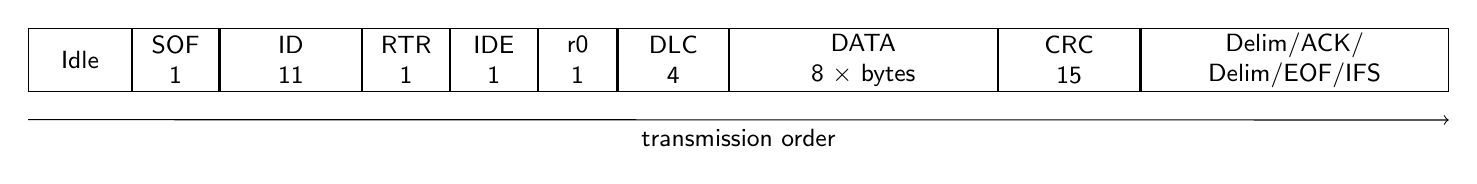
\begin{tikzpicture}[field/.style={draw, minimum height=0.8cm, align=center, font=\small, inner sep=1.5pt}]
\node[field, minimum width=1.3cm] (idle1) {Idle};
\node[field, minimum width=1.1cm, right=0pt of idle1] (sof) {SOF\\1};
\node[field, minimum width=1.8cm, right=0pt of sof] (id) {ID\\11};
\node[field, minimum width=1.1cm, right=0pt of id] (rtr) {RTR\\1};
\node[field, minimum width=1.1cm, right=0pt of rtr] (ide) {IDE\\1};
\node[field, minimum width=1.0cm, right=0pt of ide] (r0) {r0\\1};
\node[field, minimum width=1.4cm, right=0pt of r0] (dlc) {DLC\\4};
\node[field, minimum width=3.4cm, right=0pt of dlc] (data) {DATA\\8 $\times$ bytes};
\node[field, minimum width=1.8cm, right=0pt of data] (crc) {CRC\\15};
\node[field, minimum width=3.9cm, right=0pt of crc] (tail) {Delim/ACK/\\Delim/EOF/IFS};
\draw[->] ([yshift=-0.35cm]idle1.south west) -- node[below, font=\small]{transmission order} ([yshift=-0.35cm]tail.south east);
\end{tikzpicture}
\end{center}}

% Header matching the quiz layout, with an "Answer Key" label in place of the Name/Date fields.
\newcommand{\solutionsHeader}{%
\noindent
\begin{minipage}[t]{\dimexpr\textwidth-2\gradeCircleRadius-0.5in\relax}
    {\large\textbf{ECGR 4101/5101 --- Advanced Embedded Systems}}\par
    \textbf{Quiz 1: USB and CAN Bus --- Version \quizVersion\ (Solutions Guide)}\\[8pt]
    \textbf{Answer Key}
\end{minipage}%
\hfill
\raisebox{0.15in}{%
\begin{minipage}[t]{\dimexpr 2\gradeCircleRadius+0.2in\relax}
    \centering
    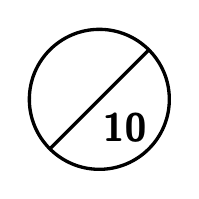
\begin{tikzpicture}[baseline=(circtop.base)]
        \coordinate (circtop) at (0,\gradeCircleRadius);
        \draw[very thick] (0,0) circle (\gradeCircleRadius);
        \draw[very thick] ({\gradeCircleRadius*cos(225)},{\gradeCircleRadius*sin(225)}) -- ({\gradeCircleRadius*cos(45)},{\gradeCircleRadius*sin(45)});
        \node at ({0.36*\gradeCircleRadius},{-0.4*\gradeCircleRadius}) {\Large\textbf{10}};
    \end{tikzpicture}
\end{minipage}}

\vspace{0.1in}
\textit{The correct choice for each question is shown in \sol{red}.}

\vspace{0.1in}
}

\pagestyle{empty}

\begin{document}

%%%%%%%%%%%%%%%%%%%%%%%%%%%%%%%%%%%%%%%%%%%%%%%%%%%%%%%%%%%%%%%%%%%%%%%%%%%%%%
\renewcommand{\quizVersion}{A}
\solutionsHeader

\begin{enumerate}[label=\textbf{\arabic*.}, leftmargin=*, itemsep=8pt]

\item \textbf{(5 points)} The figure below is a capture of the D+ and D- lines during a single USB data packet.

\begin{center}
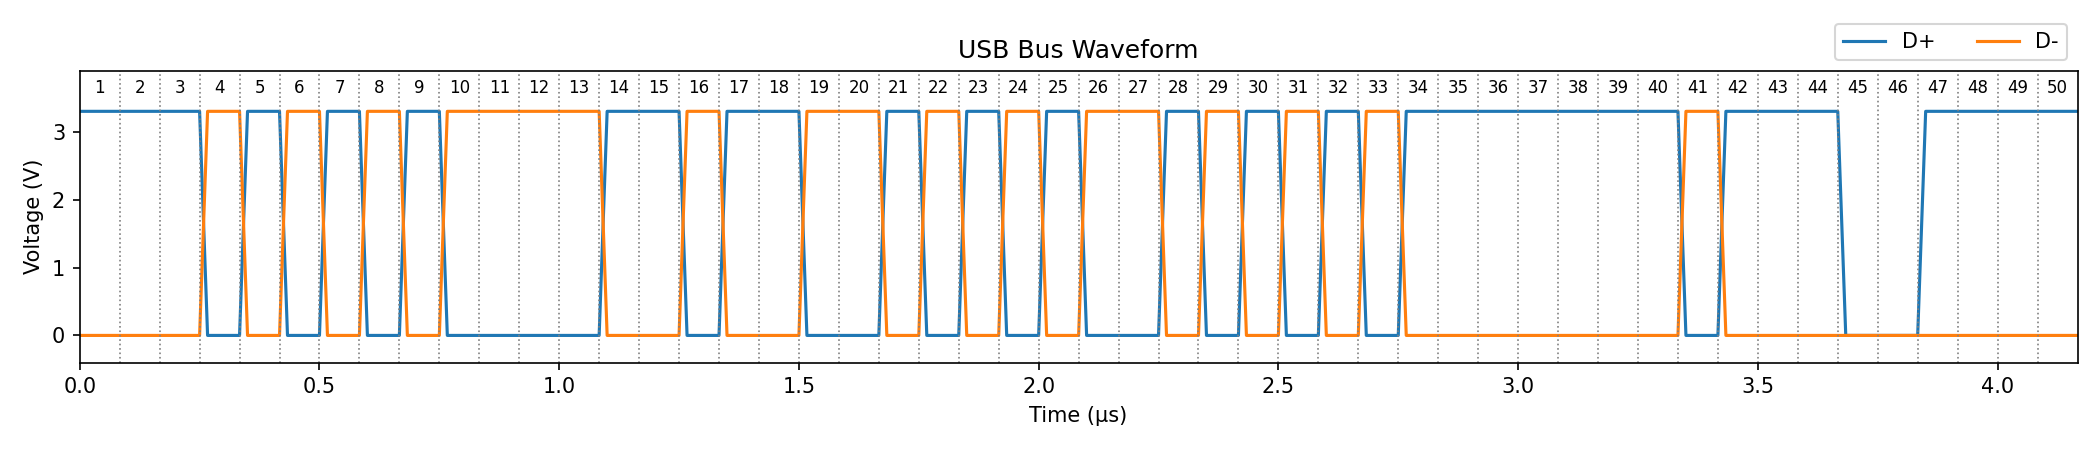
\includegraphics[width=\linewidth]{versionA/usb_waveform.png}
\end{center}
\usbFrameDiagram

\begin{enumerate}[label=(\alph*), leftmargin=*, itemsep=6pt]
\item \textbf{(2 points)} Is this a low-speed or full-speed USB packet?

\centerline{\textbf{(A)} Low-speed (1.5 Mbit/s) \qquad \sol{\textbf{(B)} Full-speed (12 Mbit/s)} \qquad \textbf{(C)} High-speed (480 Mbit/s) \qquad \textbf{(D)} Cannot be determined}
\sol{The waveform spans about 4.2 \textmu s for 50 bit times, giving a bit time of about 83 ns, matching full-speed USB's 12 Mbit/s rate.}

\item \textbf{(2 points)} Which SYNC field bit pattern (bit times 4--11) is correct?

\centerline{\sol{\textbf{(A)} 00000001} \qquad \textbf{(B)} 10000000 \qquad \textbf{(C)} 01111111 \qquad \textbf{(D)} 11111110}
\sol{SYNC is a fixed field; it always decodes to \texttt{00000001}, which this waveform confirms.}

\item \textbf{(1 point)} Which bit time(s) contain a bit-stuffing bit?

\centerline{\textbf{(A)} bit 34 \qquad \sol{\textbf{(B)} bit 41} \qquad \textbf{(C)} bits 27 and 41 \qquad \textbf{(D)} none}
\sol{One stuff bit is inserted at bit time 41, inside the CRC16 field, after six consecutive \texttt{1} bits.}
\end{enumerate}

\item \textbf{(5 points)} The figure below is a capture of the CAN\_H and CAN\_L lines during a single standard-frame CAN data frame.

\begin{center}
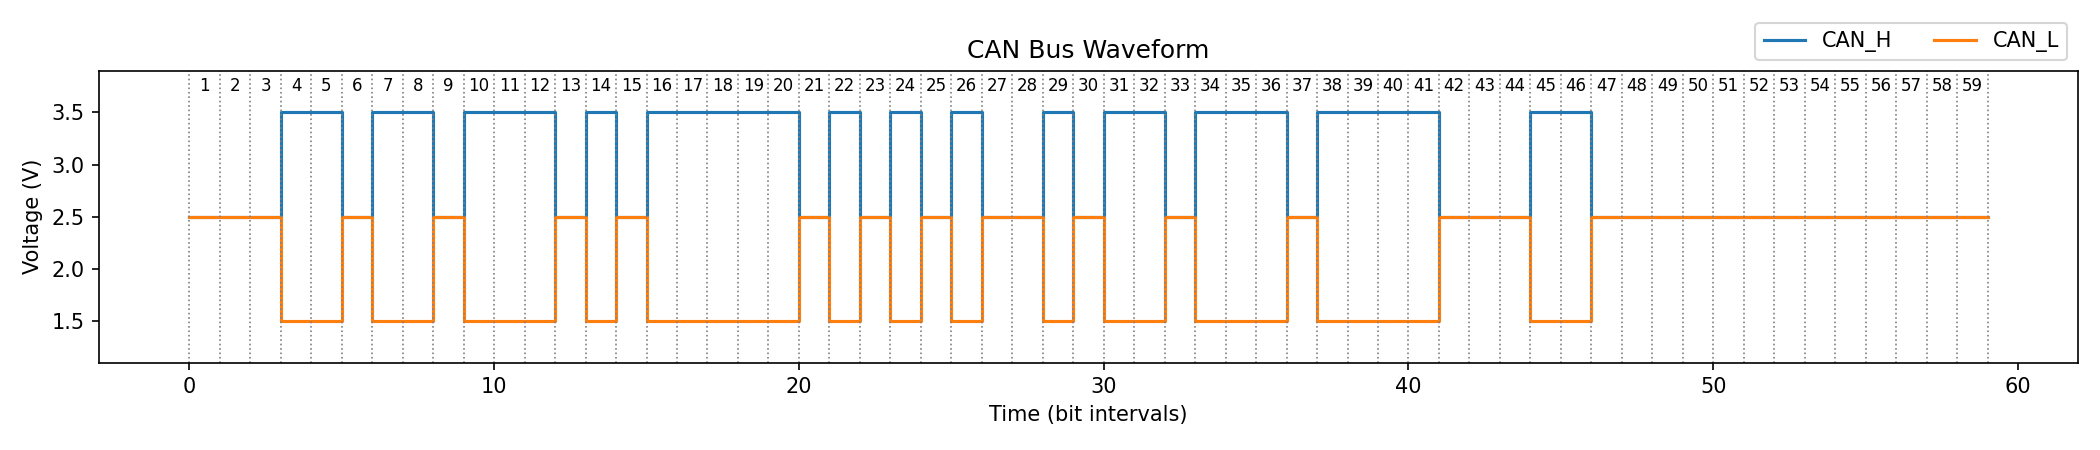
\includegraphics[width=\linewidth]{versionA/can_waveform.png}
\end{center}
\canFrameDiagram

\begin{enumerate}[label=(\alph*), leftmargin=*, itemsep=6pt]
\item \textbf{(1 point)} On the physical bus, a dominant bit corresponds to which logic level?

\centerline{\textbf{(A)} Logic 1 \qquad \sol{\textbf{(B)} Logic 0} \qquad \textbf{(C)} High impedance \qquad \textbf{(D)} Depends on the transmitting node}

\item \textbf{(1 point)} Which bit time(s) contain a bit-stuffing bit?

\centerline{\textbf{(A)} bit 14 \qquad \sol{\textbf{(B)} bit 21} \qquad \textbf{(C)} bits 14 and 21 \qquad \textbf{(D)} none}
\sol{One stuff bit is inserted at bit time 21, inside the DLC field, after five consecutive identical bits.}

\item \textbf{(1 point)} How many data bytes does this frame carry?

\centerline{\sol{\textbf{(A)} 1} \qquad \textbf{(B)} 2 \qquad \textbf{(C)} 3 \qquad \textbf{(D)} 4}
\sol{The DLC field decodes to \texttt{0001}, i.e.\ 1 data byte.}

\item \textbf{(1 point)} Decode the 11-bit identifier carried by this frame. Give your answer in hex.

\centerline{\sol{\textbf{(A)} 0x245} \qquad \textbf{(B)} 0x244 \qquad \textbf{(C)} 0x645 \qquad \textbf{(D)} 0x225}
\sol{The 11 identifier bits decode to \texttt{010 0100 0101}, i.e.\ 0x245.}

\item \textbf{(1 point)} If we have two identifiers that were transmitted at the same time, which one would be placed on the bus?

\centerline{\sol{\textbf{(A)} The identifier with the numerically lower value} \qquad \textbf{(B)} The identifier with the numerically higher value}
\centerline{\textbf{(C)} Whichever node started transmitting first \qquad \textbf{(D)} Both are placed on the bus simultaneously}
\sol{A lower identifier has more leading \texttt{0}s (dominant bits). During arbitration, as soon as one node transmits a recessive (\texttt{1}) bit while another transmits dominant (\texttt{0}), the node sending the \texttt{1} loses and stops transmitting --- so the numerically lower identifier wins the bus.}
\end{enumerate}

\end{enumerate}

\newpage

%%%%%%%%%%%%%%%%%%%%%%%%%%%%%%%%%%%%%%%%%%%%%%%%%%%%%%%%%%%%%%%%%%%%%%%%%%%%%%
\renewcommand{\quizVersion}{B}
\solutionsHeader

\begin{enumerate}[label=\textbf{\arabic*.}, leftmargin=*, itemsep=8pt]

\item \textbf{(5 points)} The figure below is a capture of the D+ and D- lines during a single USB data packet.

\begin{center}
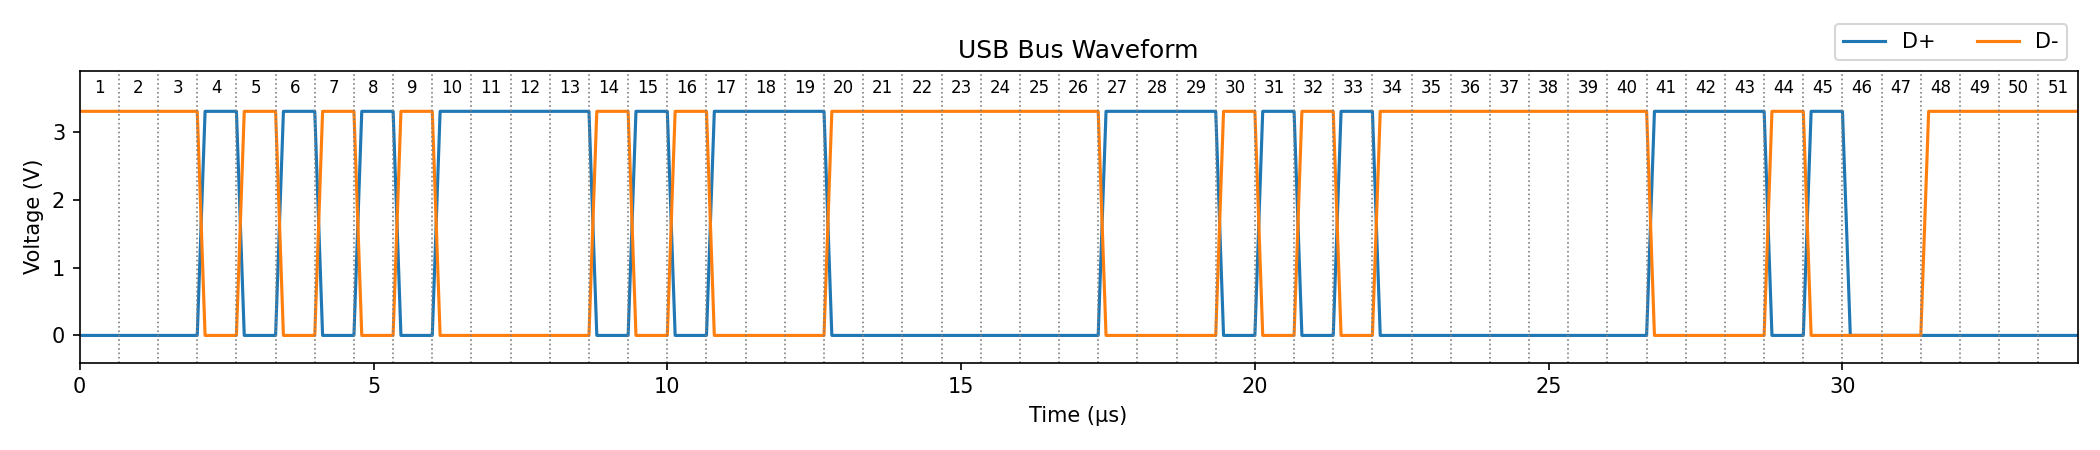
\includegraphics[width=\linewidth]{versionB/usb_waveform.png}
\end{center}
\usbFrameDiagram

\begin{enumerate}[label=(\alph*), leftmargin=*, itemsep=6pt]
\item \textbf{(2 points)} Is this a low-speed or full-speed USB packet?

\centerline{\textbf{(A)} Full-speed (12 Mbit/s) \qquad \textbf{(B)} High-speed (480 Mbit/s) \qquad \sol{\textbf{(C)} Low-speed (1.5 Mbit/s)} \qquad \textbf{(D)} Cannot be determined}
\sol{The waveform spans about 34 \textmu s for 51 bit times, giving a bit time of about 667 ns, matching low-speed USB's 1.5 Mbit/s rate.}

\item \textbf{(2 points)} Which SYNC field bit pattern (bit times 4--11) is correct?

\centerline{\textbf{(A)} 11111110 \qquad \textbf{(B)} 01111111 \qquad \sol{\textbf{(C)} 00000001} \qquad \textbf{(D)} 10000000}
\sol{SYNC is a fixed field; it always decodes to \texttt{00000001}, which this waveform confirms.}

\item \textbf{(1 point)} Which bit time(s) contain a bit-stuffing bit?

\centerline{\textbf{(A)} bit 41 only \qquad \textbf{(B)} bit 27 only \qquad \sol{\textbf{(C)} bits 27 and 41} \qquad \textbf{(D)} none}
\sol{Two stuff bits are inserted, at bit times 27 (inside DATA) and 41 (inside CRC16), each after six consecutive \texttt{1} bits.}
\end{enumerate}

\item \textbf{(5 points)} The figure below is a capture of the CAN\_H and CAN\_L lines during a single standard-frame CAN data frame.

\begin{center}
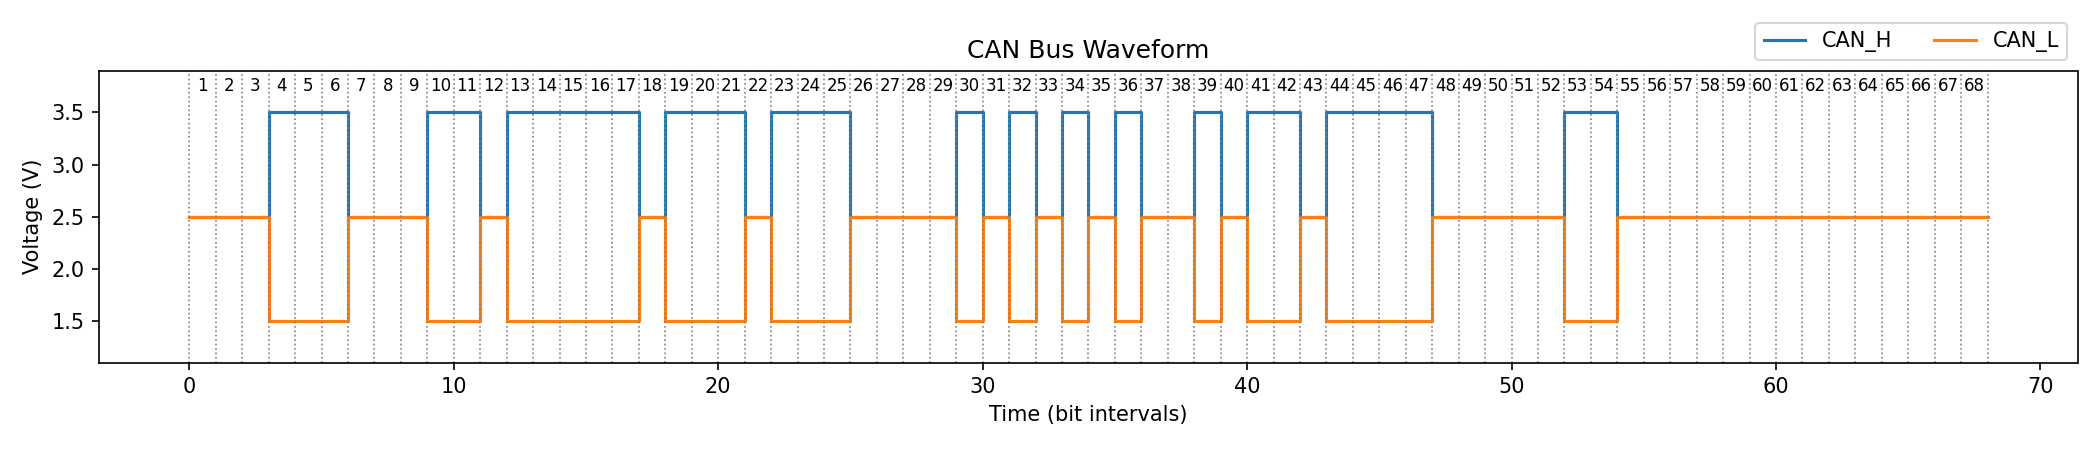
\includegraphics[width=\linewidth]{versionB/can_waveform.png}
\end{center}
\canFrameDiagram

\begin{enumerate}[label=(\alph*), leftmargin=*, itemsep=6pt]
\item \textbf{(1 point)} On the physical bus, a dominant bit corresponds to which logic level?

\centerline{\textbf{(A)} High impedance \qquad \textbf{(B)} Depends on the transmitting node \qquad \textbf{(C)} Logic 1 \qquad \sol{\textbf{(D)} Logic 0}}

\item \textbf{(1 point)} Which bit time(s) contain a bit-stuffing bit?

\centerline{\textbf{(A)} bit 18 only \qquad \textbf{(B)} bit 53 only \qquad \sol{\textbf{(C)} bits 18 and 53} \qquad \textbf{(D)} none}
\sol{Two stuff bits are inserted, at bit times 18 (between IDE and r0) and 53 (inside CRC), each after five consecutive identical bits.}

\item \textbf{(1 point)} How many data bytes does this frame carry?

\centerline{\textbf{(A)} 4 \qquad \textbf{(B)} 1 \qquad \sol{\textbf{(C)} 2} \qquad \textbf{(D)} 3}
\sol{The DLC field decodes to \texttt{0010}, i.e.\ 2 data bytes.}

\item \textbf{(1 point)} Decode the 11-bit identifier carried by this frame. Give your answer in hex.

\centerline{\textbf{(A)} 0x1A8 \qquad \textbf{(B)} 0x5C8 \qquad \sol{\textbf{(C)} 0x1C8} \qquad \textbf{(D)} 0x1C9}
\sol{The 11 identifier bits decode to \texttt{001 1100 1000}, i.e.\ 0x1C8.}

\item \textbf{(1 point)} If we have two identifiers that were transmitted at the same time, which one would be placed on the bus?

\centerline{\textbf{(A)} Whichever node started transmitting first \qquad \textbf{(B)} Both are placed on the bus simultaneously}
\centerline{\sol{\textbf{(C)} The identifier with the numerically lower value} \qquad \textbf{(D)} The identifier with the numerically higher value}
\sol{A lower identifier has more leading \texttt{0}s (dominant bits). During arbitration, as soon as one node transmits a recessive (\texttt{1}) bit while another transmits dominant (\texttt{0}), the node sending the \texttt{1} loses and stops transmitting --- so the numerically lower identifier wins the bus.}
\end{enumerate}

\end{enumerate}

\end{document}
